\chapter{Continuità dei campi}

\begin{figure}[h]
    \centering
    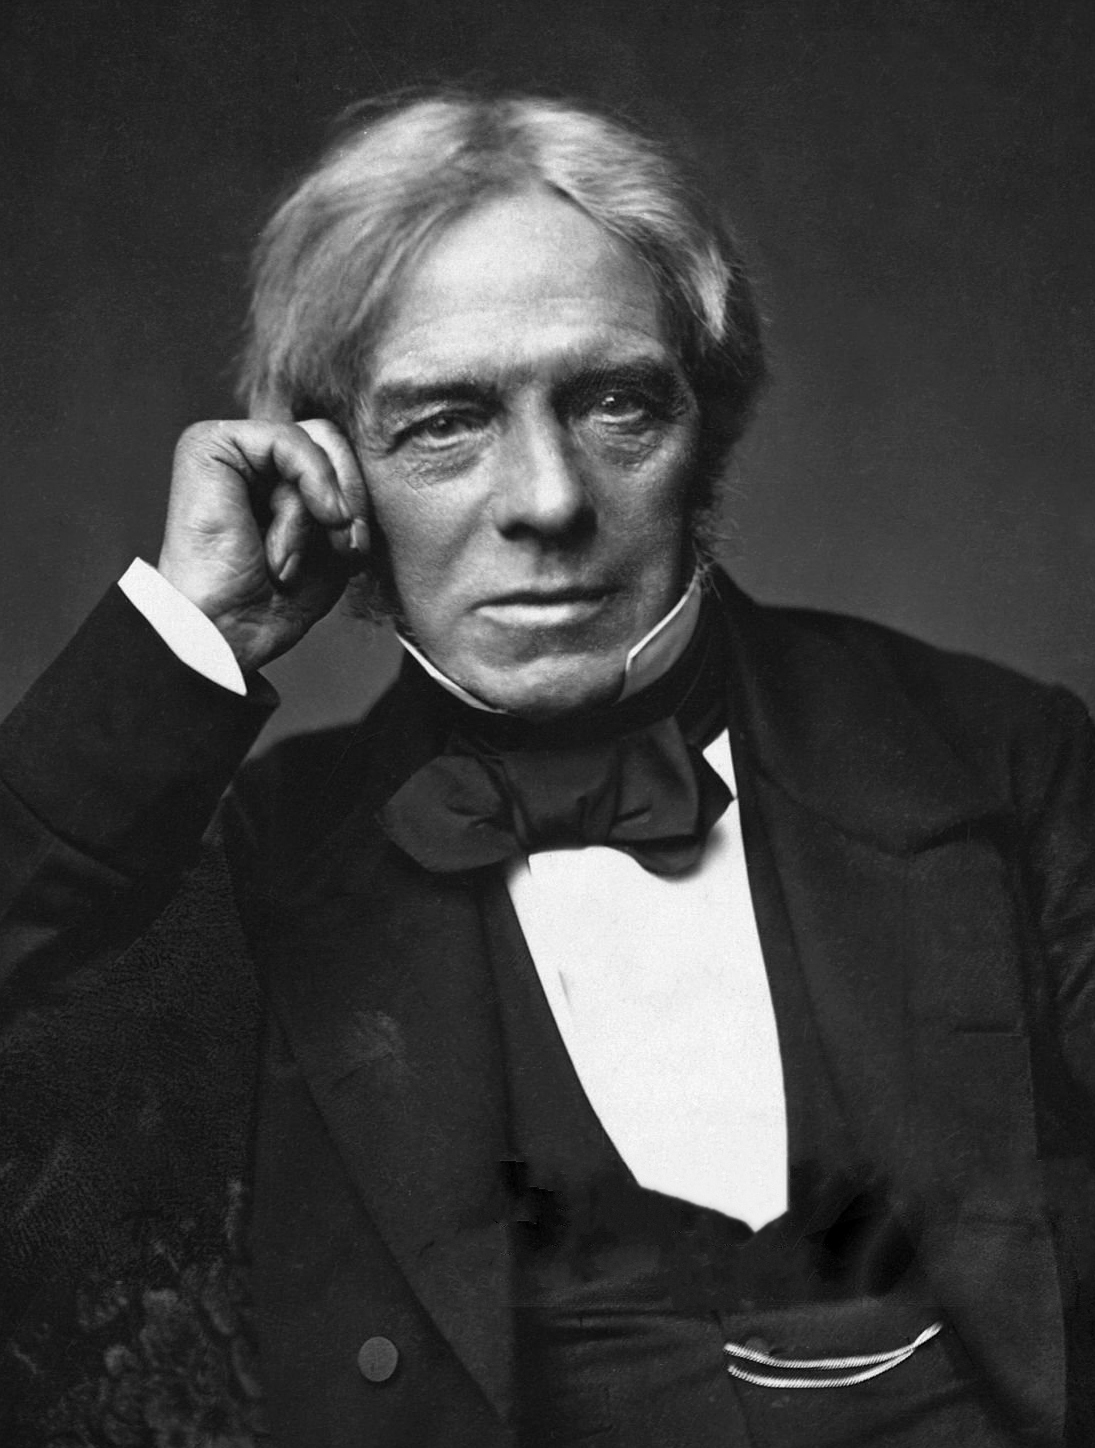
\includegraphics{Michael_Faraday_sitting_crop.jpg} 
\end{figure} 


\begin{figure}[h]
    \centering
    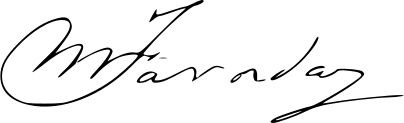
\includegraphics[scale = 0.8]{Michael_Faraday_signature.png} 
\end{figure}  

\newpage 

\section{Continuità dei campi in un confine} 

\footnote{FWC - pag 145 | 3.14 Continuity conditions for AC fields at a boundary: uniqueness of solutions} 

\begin{figure}[h]
    \centering
    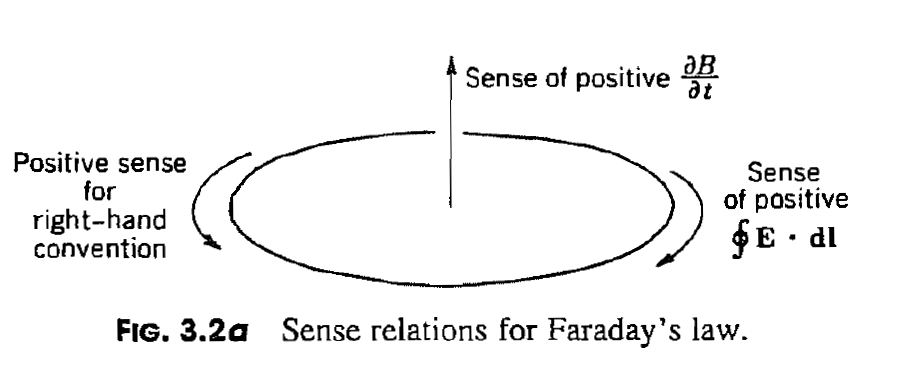
\includegraphics[scale = 0.8]{Faraday's law.PNG} 
\end{figure}  

\footnote{FWC - pag 117} 

Dalle leggi di Maxwell sappiamo che, la legge di Faraday da forma vettoriale a forma integrale è: 

{
    \Large
    \begin{equation}
        \nabla \times \vec{E} = \oint \vec{E} \cdot \vec{dl}      
    \end{equation}
}

\begin{figure}[h]
    \centering 
    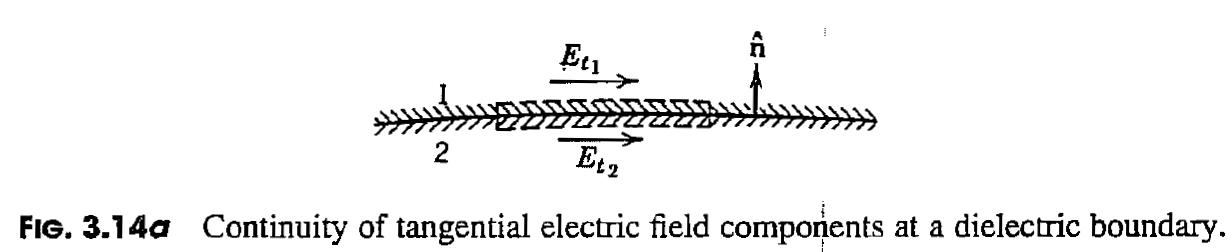
\includegraphics[scale = 0.6]{Continuity of E in a boundary.PNG}
\end{figure} 

\footnote{FWC - pag 146} 

Il confine divide due regioni di campo (nella figura indicati come 1 e 2). \\ 

Essendo $\vec{E}$ un campo conservativo, possiamo scegliere il percorso chiuso: prenderemo un rettangolo. \\ 





Quindi, considerando il senso orario, l'integrale di linea sul percorso chiuso (detto anche circuitazione) scelto: \\ 

{\Large \begin{equation}
    \oint \vec{E} \cdot \vec{dl} = (E_{T1} - E_{T2}) \Delta l
\end{equation}}

dove: \\

$E_{T1}$ è la proiezione di $\vec{E}$ del campo 1 lungo il confine \\ 
$E_{T2}$ è la proiezione di $\vec{E}$ del campo 2 lungo il confine \\ 
$\Delta l$ è la distanza infinitesima (cioè che tende a zero) tra $E_{T1}$ e $E_{T2}$ \\ \\ 


Siccome $\vec{dl}$ tende a zero: 

{\Large \begin{equation}
    \begin{cases}
    \oint \vec{E} \cdot \vec{dl} = 0 
    \Rightarrow (E_{T1} - E_{T2}) \Delta l = 0
    \Rightarrow E_{T1} = E_{T2} \\ 
    -\frac{\partial \vec{B}}{\partial t} = 0 
    \end{cases}
\end{equation}}


Possiamo consideraro lo stesso procedimento, ma per la legge di Ampere per un confine privo di cariche: 

{\Large \begin{equation}
    \begin{cases}
        \nabla \times \vec{H} = 0 
        \Rightarrow (H_{T1} - H_{T2}) \Delta l = 0 
        \Rightarrow H_{T1} = H_{T2} \\ 
        \vec{J} = 0 \\ 
        \varepsilon \frac{\partial B}{\partial t} = 0     
    \end{cases}
\end{equation}}

Considerando il versore $\hat{n}$ perpendicolare al confine, possiamo scrivere, in forma vettoriale: 

{\Large \begin{equation}
    \begin{cases}
        \hat{n} \times (\vec{E_1} -\vec{E_2} ) = 0 \\
        \hat{n} \times (\vec{H_1} - \vec{H_2}) = 0 
    \end{cases}
\end{equation}}

Quindi, per esserci continuità tra due materiali, le componenti tangenziali di $\vec{E}$ e $\vec{H}$ 
nei due materiali devono essere uguali. \\ \\ 

I passaggi visti per la legge di Ampere-Maxwell e la legge di Faraday al confine, possono essere applicati anche 
alle leggi di Gauss elettrica e legge di Gauss magnetica, considerando un'area infintesima $\Delta s$, piuttosto che un $\Delta l$ e un confine privo di caiche. \\ 

\begin{figure}[h]
    \centering 
    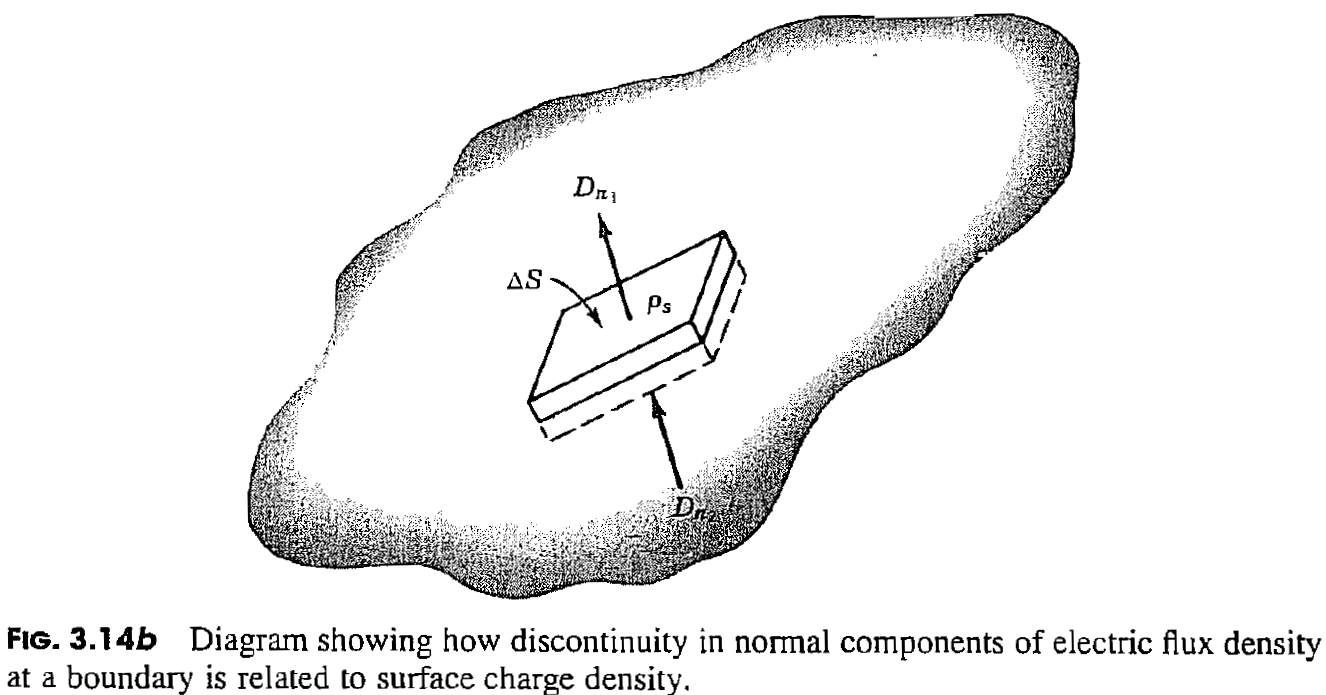
\includegraphics[scale = 0.6]{Electric flux density at a boundary.PNG}
\end{figure} 

\footnote{FWC - pag 147}


Considerando la legge di Gauss elettrica: 

{\Large \begin{equation} 
    \begin{split}
        \nabla \cdot \vec{D} = \rho  
        &\Rightarrow \Delta S (D_{n1} - D_{n2}) = \rho_s \Delta S 
        \\
        &\Rightarrow D_{n1} - D_{n2} = \rho_s\\ 
        &\Rightarrow D_{n1} - D_{n2} = 0 \\
        &\Rightarrow D_{n1} = D_{n2} \\
        &\Rightarrow \varepsilon_1 E_{n1} = \varepsilon_2 E_{n2}
    \end{split} 
\end{equation}}

Quindi, per un confine senza cariche, i componenti di $\vec{E}$ perpendicolari alla superficie sono continui, mentre sono discontinui quando in 
un confine sono presenti delle cariche. \\ 

Considerando la legge di Gauss magnetica: 

{\Large \begin{equation}
    \begin{split}
    \nabla \cdot \vec{B} = 0  
    &\Rightarrow \Delta S (B_{n1} - B_{n2}) = 0 \\
    &\Rightarrow B_{n1} - B_{n2} = 0 \\ 
    &\Rightarrow B_{n1} = B_{n2} \\ 
    &\Rightarrow \mu_1 H_{n1} = \mu_2 H_{n2}
    \end{split}
\end{equation}}

\newpage 

\section{Continuità dei campi in un confine di un conduttore perfetto }
\footnote{FWC - pag 148 | Bounday conditions at a perfect conductor for AC fields} 

In un conduttore perfetto: 
{
    \Large
    \begin{equation}
    E_{T2} = 0       
    \end{equation}
}

Dal capitolo precedente, sappiamo che: 

{
    \Large
    \begin{equation}
    E_{T1} = E_{T2} \Rightarrow E_{T1} = 0        
    \end{equation}
}

quindi anche fuori dal conduttore. \\ 

Per lo stessso principio: 

{
    \Large
    \begin{equation}
    D_{n2} = 0       
    \end{equation}
}


\begin{figure}[h]
    \centering 
    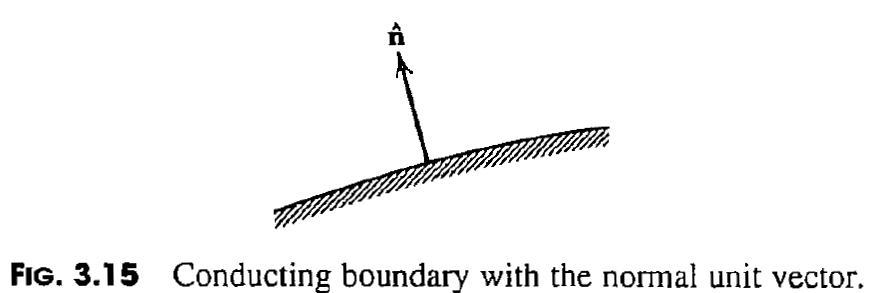
\includegraphics[scale = 0.6]{Boundary in a perfect conductor.PNG}
\end{figure} 

\footnote{FWC - pag 149}

{\Large \begin{equation}
    \begin{split}
        \nabla \times \vec{B} 
        = \vec{J} 
        &\Rightarrow \oint \vec{H} \cdot \vec{dl} 
        = \oint \vec{J} \cdot \vec{dl}
        \\ 
        &\Rightarrow H_t dl = J_s dl
        \\
        &\Rightarrow H_t = J_s    
    \end{split}
\end{equation}}
Quindi, in un conduttore perfetto: 

{\Large \begin{equation}
    \begin{cases}
        \hat{n} \times \vec{E} = 0 \\ 
        \hat{n} \cdot \vec{B} = 0 \\ 
        \rho_s = \hat{n} \cdot \vec{D} \\ 
        \vec{J_s} = \hat{n} \times \vec{H}
    \end{cases}
\end{equation}}



